\documentclass{beamer}
\usefonttheme{professionalfonts}  % serif math
\setbeamertemplate{frametitle continuation}{} %{(\insertcontinuationcount)}

\iffalse
\usepackage{pgfpages}
\setbeameroption{show notes}
\setbeameroption{show notes on second screen=right}
% pdfpc slajdovi.pdf --notes=right
\fi

\usepackage[scaled]{beramono}				% sans-serif monospace
% font
\renewcommand{\familydefault}{\sfdefault}  % sans-serif main

%\usepackage{arev}
%\usepackage[cm]{sfmath}  % bolje nego mathastext
%\SetSymbolFont{largesymbols}{normal}{OMX}{iwona}{m}{n}

%\usepackage[italic]{mathastext}  % sfmath je bolje (manji indeksi)


%\usepackage{inconsolata}					% sans-serif monospace
\usepackage[scaled]{beramono}				% sans-serif monospace


%\usepackage[math]{iwona}
%\usepackage[math]{kurier}
%\usepackage[T1]{fontenc}  % accented characters, copy from pdf, ...

\raggedright						% bez desnog poravnavanja

\usepackage{caption}
\captionsetup{%
	justification=raggedright,
}
\setlength{\parindent}{1em}	 % uvlačenje ulomaka
\usepackage{indentfirst}	 % uvlačenje prvog ulomka
\setlength{\parskip}{0.5em}	 % razmak između ulomaka

\usepackage{listings}  % listings
\renewcommand{\lstlistingname}{Ispis}

\usepackage[multiple]{footmisc}	 % višestruke fusnote

\usepackage[hidelinks]{hyperref}
\renewcommand*{\UrlFont}{\footnotesize}

% colors

\usepackage{xcolor}
\usepackage{color}

\hypersetup{
	colorlinks,
	linkcolor={blue!50!green!50!black},  % xcolor package
	citecolor={green!40!black},
	urlcolor={blue!75!green!30!black}
}
\definecolor{bluekeywords}{rgb}{0.13,0.13,1}  % color package
\definecolor{greencomments}{rgb}{0,0.5,0}
\definecolor{redstrings}{rgb}{0.9,0,0}

\let\emph\relax
\DeclareTextFontCommand{\emph}{\bfseries}

\newtheorem{theorem}{Teorem}[section]
\newtheorem{definition}{Definicija}[section]

\usepackage{enumitem}  % \begin{enumerate}[topsep=0pt,itemsep=0pt,partopsep=0pt]

%%text%%
\iftrue
	\raggedright						% bez desnog poravnavanja
	\raggedbottom
	\usepackage{caption}
	\captionsetup{%
		justification=raggedright,
	}
	\usepackage{etoolbox}
	\makeatletter
	\patchcmd{\@dottedtocline}
	{\rightskip\@tocrmarg}
	{\rightskip\@tocrmarg plus 4em \hyphenpenalty\@M}
	{}{}
	\makeatother
	\setlength{\parindent}{1em}	 % uvlačenje ulomaka
	\usepackage{indentfirst}	 % uvlačenje prvog ulomka
	\setlength{\parskip}{0.5em}	 % razmak između ulomaka
	
	\usepackage[multiple, bottom]{footmisc}	 % višestruke fusnote, poslije slika/tablica
	
	\renewcommand*{\UrlFont}{\footnotesize}
	
	% colors	
	\iffalse
	\usepackage{xcolor}
	\usepackage{color}
	\hypersetup{
		colorlinks,
		linkcolor={blue!60!green!50!black},  % xcolor package
		citecolor={green!40!black},
		urlcolor={blue!75!green!30!black}
	}
	\definecolor{bluekeywords}{rgb}{0.13,0.13,1}  % color package
	\definecolor{greencomments}{rgb}{0,0.5,0}
	\definecolor{redstrings}{rgb}{0.9,0,0}
	\fi
	
	\DeclareTextFontCommand{\textbf}{\bfseries}
\fi
%%%%%%%%
% redefinition of left and right to make spacing consistent
\let\originalleft\left
\let\originalright\right
\def\left#1{\mathopen{}\originalleft#1}
\def\right#1{\originalright#1\mathclose{}}

\usepackage{amsmath}
\usepackage{mathtools}  % \coloneqq
%\usepackage{bm}
%\usepackage[utopia]{mathdesign}
\usepackage[OMLmathsfit]{isomath}  % \DeclareMathAlphabet ...
%\usepackage[bbgreekl]{mathbbol}

\usepackage{mathtools}  % smashoperator
\usepackage{commath}  % calculus, perentheses
\usepackage{stmaryrd}  % \llbracket for \rrbracket, ...

%\usepackage[croatian]{babel}		% teorem
%\newtheorem{definition}{Definicija}[section]
%\newtheorem{theorem}{Teorem}[section]
%\newtheorem{corollary}{Korolar}[theorem]

\DeclareMathAlphabet{\mathbbmsl}{U}{bbm}{m}{sl}
\DeclareMathAlphabet{\mathbbmb}{U}{bbm}{b}{it}
\DeclareMathAlphabet{\mathbbmssit}{U}{bbmss}{m}{it}


% common set?, distribution
\newcommand{\commset}[1]{\mathbbmb{#1}}
\newcommand{\distrib}[1]{\mathcal{#1}}

% sans-serif blackboard-bold
\newcommand{\mathsfbbit}[1]{\mathbbmssit{#1}}

% variable
\let\vec\relax
\let\set\relax
\newcommand{\vec}[1]{\mathbfit{#1}}
\newcommand{\mat}[1]{\vec{#1}}
\newcommand{\ten}[1]{\vec{#1}}
\newcommand{\set}[1]{\mathbbmsl{#1}}

% constant
\newcommand{\const}[1]{\mathrm{#1}}
\newcommand{\cvec}[1]{\mathbf{#1}}
\newcommand{\cmat}[1]{\cvec{#1}}
\newcommand{\cten}[1]{\cvec{#1}}
\newcommand{\cset}[1]{\mathbb{#1}}

% random variable
\newcommand{\rvar}[1]{{\color{blue!70!black}\mathsfit{#1}}}
\newcommand{\rvec}[1]{{\color{blue!70!black}\mathsfbfit{#1}}}
\newcommand{\rmat}[1]{\rvec{#1}}
\newcommand{\rten}[1]{\rvec{#1}}
\newcommand{\rset}[1]{{\color{blue!70!black}\mathsfbbit{#1}}}

% linear algebra
\newcommand{\transpose}{\mathsf T}

% calculus - commath: od, pd, md, dif
% parentheses - commath: del, cbr, sbr, envert, enVert

% named functions
\DeclareMathOperator{\softplus}{softplus}
\DeclareMathOperator{\softmax}{softmax}
\DeclareMathOperator{\logistic}{\sigma}
\DeclareMathOperator{\sgn}{sgn}
\DeclareMathOperator{\diag}{diag}

% operators
\DeclareMathOperator*{\argmin}{arg\,min} % thin space
\DeclareMathOperator*{\argmax}{arg\,max}
\DeclareMathOperator*{\E}{{\rm I\kern-.282em E}}
\DeclareMathOperator*{\D}{{\rm I\kern-.282em D}}
\DeclareMathOperator*{\Cov}{Cov}
\let\H\relax
\DeclareMathOperator*{\H}{{\rm H\kern-.8em H}}
\DeclareMathOperator*{\Dklsym}{D_{\mathrm{KL}}}

% bracket operators
\newcommand{\enangle}[1]{\mathinner{\left\langle{#1}\right\rangle}}
\newcommand{\enbbracket}[1]{\mathinner{\left\llbracket{#1}\right\rrbracket}}
\newcommand{\braket}[2]{\enangle{{#1}|{#2}}}

% parentheses from commath redefined to improve spacing because (left and right were redefined)
\renewcommand{\del}[1]{\left(#1\right)}
\renewcommand{\sbr}[1]{\left[#1\right]}
\renewcommand{\cbr}[1]{\left\{#1\right\}}
\renewcommand{\intoo}[1]{\mathinner{\del{#1}}}
\renewcommand{\intcc}[1]{\mathinner{\sbr{#1}}}
\renewcommand{\intco}[1]{\mathinner{\left[#1\right)}}
\renewcommand{\intoc}[1]{\mathinner{\left(#1\right]}}

% special
\newcommand{\funcdef}[3]{#1 \colon #2 \to #3}
\newcommand{\Dkl}[2]{\Dklsym\del{#1\;\middle\|\;#2}}
\newcommand{\C}{\cset{C}}
\newcommand{\R}{\cset{R}}
\newcommand{\Z}{\cset{Z}}
\newcommand{\N}{\cset{N}}
\newcommand{\dirac}{\delta}
\newcommand{\ind}[2]{#1_{\sbr{#2}}}

% operators
\newcommand{\bidot}{\mkern1.5mu{..}\mkern1.5mu}
\newcommand\sheq{\mkern1.5mu{=}\mkern1.5mu}
%\renewcommand{\dots}{...}
\usepackage{booktabs}  % from the tamplate; table quality enhancement

\usepackage{multirow}
\usepackage{tabularx}

\newcolumntype{P}[1]{>{\raggedright\let\newline\\\arraybackslash\hspace{0pt}}p{#1}}

\renewcommand{\arraystretch}{1.4}
%\usepackage{floatrow} 				% centriranje svih slika
\usepackage{float}					% figure [H]
\usepackage{graphicx} 				% includegraphics
\usepackage{caption}			% subfigure
\usepackage{subcaption}			% subfigure
\usepackage[export]{adjustbox} 	% http://ctan.org/pkg/adjustbox

\usepackage[section]{placeins}  % [section] for \FloatBarrier before every section 

\graphicspath{ {./figures/} }		% mapa sa slikama
%\let\oldincludegraphics\includegraphics
%\renewcommand{\includegraphics}[2][]{\oldincludegraphics[#1,max width=0.9\linewidth]{#2}}

%\usepackage{flafter} % floats after the first reference

\usepackage{tikz} 					% dijagrami
\usepackage{pgfplots}
\usetikzlibrary{fit,automata,arrows,positioning,calc,petri,topaths,arrows.meta}

%\usetikzlibrary{external}
%\tikzexternalize[prefix=figures/tikz/, shell escape=-enable-write18]
%TexStudio Configuration\commands\pdflatex:
%"pdflatex.exe -src -interaction=nonstopmode --shell-escape %.tex

\pgfplotsset{every axis/.append style={
		axis x line=middle,    	% put the x axis in the middle
		axis y line=middle,    	% put the y axis in the middle
		axis line style={->},  	% arrows on the axis
		xlabel={$x$},          	% default put x on x-axis
		ylabel={$y$},          	% default put y on y-axis
		samples=100,
		axis equal,
}} % axis style

\tikzset{
	>={Triangle[length=1.8mm,width=1.2mm]},
	dedge/.style={arrows=->, black, thick},
}
% PGMs
\tikzstyle{textnode} = [minimum size=5mm, node distance=9mm]
\tikzstyle{pnode} = [circle, minimum size=10mm, thick, draw=black, node distance=9mm]
\tikzstyle{greypnode} = [pnode, fill=black!5]
% https://github.com/jluttine/tikz-bayesnet
\tikzstyle{wrap} = [inner sep=0pt, fit=#1]
\tikzstyle{plate} = [draw, rectangle, rounded corners=0.5ex, thick, fit=#1]
\tikzstyle{caption} = [font=\footnotesize, node distance=0]
\tikzstyle{plate caption} = [caption, node distance=0, inner sep=0pt,
below left=5pt and 0pt of #1.south east]
\newcommand{\plate}[4][]{
	\node[wrap=#3] (#2-wrap) {};
	\node[plate caption=#2-wrap] (#2-caption) {#4};
	\node[plate=(#2-wrap)(#2-caption), #1] (#2) {};
}
% ANNs
\tikzstyle{nnode} = [circle, minimum size=10mm, thick, draw=black, node distance=5mm]
\tikzstyle{nrect} = [rectangle, minimum size=7mm, thick, draw=black, node distance=5mm, rounded corners=0.1ex]
\usepackage[croatian]{babel}		% teorem

\usepackage{dirtree}

\usepackage[]{algorithmic}

\usepackage{setspace}  % line spacing

%\usepackage{pythontex}

%\usepackage[nomessages]{fp} % fixed-point arithmetic http://ctan.org/pkg/fp

\usepackage{pdfpages} % inclusion of external pdf pages

\usepackage[toc]{appendix}

%\usepackage{natbib}
\usepackage[numbers]{natbib}
\renewcommand*{\bibfont}{\scriptsize}

\iftrue
\usepackage[croatian]{babel}
\usepackage[utf8x]{inputenc}	
\fi

\mode<presentation>
{
	\usetheme{Boadilla}      % or try Darmstadt, Madrid, Warsaw, ...
	\usecolortheme{orchid} % or try albatross, beaver, crane, ...
	\usefonttheme{structurebold}  % or try default, serif, structurebold, ...
	\setbeamertemplate{navigation symbols}{}
	\setbeamertemplate{caption}[numbered]
}
\setbeamercolor{structure}{fg=blue!75!green!80!black}	

%\setbeamertemplate{itemize items}[default]
%\setbeamertemplate{enumerate items}[default]
\setbeamertemplate{section in toc}[circle]
\setbeamertemplate{subsection in toc}[circle]
\setbeamertemplate{items}[circle]
\setbeamertemplate{blocks}[default]
\setbeamertemplate{footline}
{
	\leavevmode%
	\hbox{%
		\begin{beamercolorbox}[wd=.15\paperwidth,ht=2.25ex,dp=1ex,center]{author in head/foot}%
			%\usebeamerfont{author in head/foot}\insertshortauthor
		\end{beamercolorbox}%
		\begin{beamercolorbox}[wd=.7\paperwidth,ht=2.25ex,dp=1ex,center]{author in head/foot}%
			\usebeamerfont{title in head/foot}\insertshorttitle  %\hspace*{3em}
		\end{beamercolorbox}%
		\begin{beamercolorbox}[wd=.15\paperwidth,ht=2.25ex,dp=1ex,right]{author in head/foot}%
			\insertframenumber{} / \inserttotalframenumber\hspace*{1ex}
		\end{beamercolorbox}
	}%
	\vskip0pt%
}

\iftrue
\AtBeginSection[]
{
	\begin{frame}<beamer>
		\frametitle{Sadržaj}
		\tableofcontents[currentsection]
	\end{frame}
}
\fi


\title{Nadzirani pristupi za procjenu nesigurnosti predikcija dubokih modela}
\author{Ivan Grubišić \\ \emph{Voditelj:} Siniša Šegvić}
%\author{Voditelj: Siniša Šegvić}
\institute{Fakultet elektrotehnike i računarstva}
\date{}


\begin{document}
	
\begin{frame}
  \titlepage
\end{frame}

\begin{frame}{Sadržaj}
  \tableofcontents
\end{frame}


\section{Procjena nesigurnosti kod dubokih modela}

\begin{frame}{Procjena nesigurnosti kod dubokih modela}
	\begin{itemize}
		\item Trenutno najuspješniji modeli često pokazuju preveliku sigurnost u predikcije kod \textbf{izvanrazdiobnih} i \textbf{krivo klasificiranih} primjera \citep{Nguyen:2015:DNNEFHCPUI,Guo:2017:CMNN,Hendrycks:2016:BDMOODE}, a mogu se i pronalaziti \textbf{neprijateljski primjeri}  \citep{Szegedy:2013:IPNN,Goodfellow:2014:EHAE}.
		\item Neki oblici strojnog učenja, posebno \textbf{podržano} i \textbf{aktivno učenje} mogu imati koristi od razlikovanja je li uzrok nesigurnosti \textbf{višeznačnost podataka} ili \textbf{neznanje}, tj. nesigurnost u parametre.
		\item Složeni modeli se sve više koriste u sustavima koji donose odluke o kojima ovise sigurnost i zdravlje ljudi, pa trebaju biti sposobni pouzdano procijeniti nesigurnost/rizik.
	\end{itemize}
\end{frame}
\note[itemize]{
	\item Trenutno najuspješniji modeli često pokazuju preveliku sigurnost u predikcije kod \textbf{izvanrazdiobnih} i \textbf{krivo klasificiranih} primjera, a mogu se i pronalaziti \textbf{neprijateljski primjeri}.
	\item Neki oblici strojnog učenja, posebno \textbf{podržano} i \textbf{aktivno učenje} mogu imati koristi od razlikovanja je li uzrok nesigurnosti \textbf{višeznačnost podataka} ili \textbf{neznanje}, tj. nesigurnost u parametre
	\item Složeni modeli se sve više koriste u sustavima koji donose odluke o kojima ovise sigurnost i zdravlje ljudi, pa trebaju biti sposobni pouzdano procijeniti nesigurnost.
	\item\item 0:40 / 0:40
}

\begin{frame}{Procjena nesigurnosti kod dubokih modela}
	\begin{itemize}
		\item Nesigurnost možemo podijeliti \citep{Kiureghian:2009:AEDM} na: 
		\begin{itemize}
			\item \textbf{aleatornu nesigurnost} (lat. \textit{aleator}, \textit{kockar}) -- nesigurnost koja dolazi od višeznačnosti podataka i ne može se smanjiti zbog nedeterminizma procesa koji generira podatke,
			\item \textbf{epistemičku nesigurnost} (grč. \textit{epist\={e}m\={e}}, \textit{znanje}) ili nesigurnost modela -- nesigurnost kojoj je uzrok nedostatak znanja i može se smanjiti uz više podataka.
		\end{itemize}
		\item Granica između aleatorne i epistemičke nesigurnosti nije uvijek jasna.
		\item \textbf{Epistemička nesigurnost predikcije} proizlazi iz \textbf{nesigurnosti u parametre}, koju izražava \textbf{aposteriorna razdioba parametara} -- potrebno je \textbf{bayesovsko zaključivanje} o parametrima modela.
	\end{itemize}
\end{frame}
\note[itemize]{
	\item Nesigurnost možemo podijeliti na: 
	\begin{itemize}
		\item \textbf{aleatornu nesigurnost} (lat. \textit{aleator}, \textit{kockar}) -- nesigurnost koja dolazi od višeznačnosti podataka/nedeterminizma i ne može se smanjiti,
		\item \textbf{epistemičku nesigurnost} ili nesigurnost modela -- nesigurnost kojoj je uzrok nedostatak znanja i može se smanjiti uz više podataka.
	\end{itemize}
	\item \textbf{Epistemička nesigurnost predikcije} proizlazi iz \textbf{nesigurnosti u parametre}, koju izražava \textbf{aposteriorna razdioba parametara}.
	\item\item 0:40 / 1:20
}

\section{Izražavanje nesigurnosti predikcije}

\begin{frame}{Izražavanje nesigurnosti predikcije}
\begin{itemize}
	\item Osnovne mjere za izražavanje nesigurnosti su \textbf{vjerojatnost}, \textbf{entropija}, \textbf{diferencijalna entropija} i \textbf{varijanca}. 
	\item Neke mjere za izražavanje nesigurnosti predikcije kod klasifikacije su:
	\begin{itemize}
	 	\item vjerojatnost klase s najvećom vjerojatnošću
		\begin{align}
		\max_k \P(\rvar y=k\mid\vec x,\vec\theta)
		\end{align}
		\item entropija
		\begin{align}
		\H(\rvar y\mid\vec x,\vec\theta)=-\E_{\rvar y\mid\vec x,\vec\theta}\ln\P\del{y\mid\vec x,\vec\theta} \text{.}
		\end{align}
	\end{itemize}
	\item Ove mjere same po sebi ne razlikuju epistemičku i aleatornu nesigurnost.
\end{itemize}
\end{frame}
\note[itemize]{
	\item Neke mjere prikladne za izražavanje nesigurnosti predikcije kod klasifikacije su:
	\begin{itemize}
		\item vjerojatnost klase s najvećom vjerojatnošću
		\item entropija.
	\end{itemize}
	\item Jedan nedostatak ovih mjera je što ne razlikuju epistemičku i aleatornu nesigurnost.
	\item\item 0:20 / 1:40
}

\begin{frame}{Izražavanje nesigurnosti predikcije}
\begin{itemize}
	\item \citet{Rawat:2017:APEBDL,Smith:2018:UMUAED} kao mjeru epistemičke nesigurnosti predikcije predlažu \textbf{međusobnu informaciju između izlazne razdiobe i aposteriorne razdiobe parametara}:
	\begin{align}
	\underbrace{\I\del{\del{\rvar y\mid\vec x,\set D};\del{\rvec\theta\mid\set D}}}_{U_\text{E}}
	&= \H(\rvar y\mid\vec x,\set D) - \H\del{\del{\rvar y\mid\vec x,\set D}\mid\del{\rvec\theta\mid\set D}} \\
	&= \underbrace{\H(\rvar y\mid\vec x,\set D)}_{U} - \underbrace{\E_{\rvec\theta\mid\set D} \H(\rvar y\mid\vec x,\vec\theta)}_{U_\text{A}} \text{.} \label{eq:mi-epistemicka-nesigurnost}
	\end{align}
	\item Zadnji izraz je razlika entropije predikcije i očekivanja entropije predikcije po aposteriornoj razdiobi parametara.
	\item To se može interpretirati kao očekivano znanje o parametrima koje se dobije ako se dobije oznaka za primjer $\vec x$ (to se može bolje vidjeti ako se međusobna informacija drugačije izrazi).
\end{itemize}
\end{frame}
\note[itemize]{
	\item \citet{Rawat:2017:APEBDL,Smith:2018:UMUAED} za mjeru epistemičke nesigurnosti predikcije predlažu \textbf{međusobnu informaciju između izlazne razdiobe i aposteriorne razdiobe parametara}:
	\item (jednadžba)
	\item Ona se može izraziti kao razlika entropije predikcije i očekivanja entropije predikcije po aposteriornoj razdiobi parametara.
	\item Kao mjera ukupne nesigurnosti će se koristiti 1. član -- entropija očekivanja izlazne razdiobe po aposteriornoj razdiobi parametara.
	\item Kao mjera aleatorne nesigurnosti će se koristiti 2. član --  očekivanje entropije izlazne razdiobe po aposteriornoj razdiobi parametara.
	\item Ako se međusobna informacija drugačije izrazi, može se interpretirati kao očekivano znanje o parametrima koje se dobije ako se dobije oznaka za primjer $\vec x$.
	\item\item 1:20 / 3:00
}

%\section{Aproksimacija bayesovske neuronske mreže pomoću dropouta}

\begin{frame}{Aproksimacija bayesovske neuronske mreže pomoću dropouta}
\begin{itemize}
	\item \citet{Gal:2016:BCNNBAVI} učenje s \textit{dropoutom} interpretiraju kao varijacijsko zaključivanje.
	\item Ako pretpostavimo da \textit{dropout} dolazi iza slojeva linearne transformacije, slučajne varijable koje odgovaraju varijacijskoj razdiobi matrica težina su
	\begin{align} \label{eq:dropout-matrica-tezina}
	\rvec W_l = \diag\del{\rvec z_l}\vec M_l \text{,}
	\end{align}
	gdje je $l$ indeks sloja, $\vec M_l$ matrica varijacijskih parametara, a $\rvar z_l$ slučajni vektor čiji elementi su nezavisne slučajne varijable s Bernoullijevom razdiobom.
	\item Može se pokazati da minimizaciji $\Dkl{q_{\vec\phi}}{\p(\rvec\theta\mid\set D)}$, gdje je $q_{\vec\phi}$ varijacijska razdioba, po varijacijskim parametrima $\vec\phi$, odgovara minimizacija uobičajene funkcije pogreške kod učenja s dropoutom.
	%\begin{align}
	%E(\vec\theta;\set{D}) = -\sum_i \ln\p\del{\vec y_i\midmid\vec x_i,\rvec\theta=\tilde{\vec\theta}_i} + \frac{\lambda}{2}\sum_l\enVert{\vec M_l}_\text{F}^2 \text{.}
	%\end{align}
\end{itemize}
\end{frame}
\note[itemize]{
	\item \citet{Gal:2016:BCNNBAVI} učenje s \textit{dropoutom} interpretiraju kao varijacijsko zaključivanje.
	\item Reci matrica težina su slučajni vektori koji kao vrijednosti imaju retke matrice varijacijskih parametara $\vec M$ ili $\cvec 0^\tp$ s vjerojatnošću isključivanja.
	\item Može se pokazati da minimizaciji KL-div. između varijacijske i aposterirne razdiobe odgovara minimizacija uobičajene funkcije pogreške kod učenja s dropoutom.
	\item\item 0:40 / 3:40
}

\begin{frame}{Aproksimacija bayesovske neuronske mreže pomoću dropouta}
\begin{itemize}
	\item Obično se pri ispitivanju modela učenog s dropoutom ne koristi isključivanje jedinica, nego se parametri skaliraju vjerojatnošću neisključivanja, tj. procjenjuju se očekivanjem varijacijske razdiobe:
	\begin{align}
	p(y\mid\vec x,\set D) \approx  p\del{y\midmid\vec x,\rvec\theta=\E_{\tilde{\vec\theta}\sim q_{\vec\phi}}\tilde{\vec\theta}} \text{.}
	\end{align}
	\item Ispravniji, ali manje efikasan način usrednjavanja je očekivanje izlaza po varijacijskoj razdiobi parametara, što se može procijeniti sredinom nekog broja uzoraka izlaza uz dropout \citep{Srivastava:2014:DASWPNNO,Gal:2015:DBA} -- \textit{Monte Carlo dropout} (\textbf{MC-dropout}):
	\begin{align} \label{eq:zakljucivanje-y-bnm-q-mcd}
	\p(\vec y\mid \vec x, \set{D})
	\approx \E_{\tilde{\vec\theta}\sim q_{\vec\phi}}\p(\vec y\mid\vec x,\tilde{\vec\theta}) 
	\approx \frac{1}{M}\sum_{i=1}^M \p\del{\vec y\midmid\vec x,\rvec\theta=\tilde{\vec\theta}_i}  \text{,}
	\end{align}
	gdje su $\tilde{\vec\theta}_i$ uzorci parametara iz varijacijske razdiobe $q_{\vec\phi}$.
\end{itemize}
\end{frame}
\note[itemize]{
	\item Obično se pri ispitivanju modela učenog s dropoutom parametri skaliraju vjerojatnošću neisključivanja, tj. procjenjuju se \textbf{očekivanjem varijacijske razdiobe}.
	\item Ispravniji, ali manje efikasan način usrednjavanja je očekivanje izlaza po varijacijskoj razdiobi parametara, što se može procijeniti \textbf{sredinom nekog broja uzoraka izlaza uz dropout}.
	\item\item 0:40 / 4:20
}

\section{Prepoznavanje izvanrazdiobnih i krivo klasificiranih primjera na temelju izlaza softmaksa ili logita}

\begin{frame}{Prepoznavanje izvanrazdiobnih i krivo klasificiranih primjera na temelju izlaza softmaksa ili logita}
\begin{itemize}
	\item Razdiobe koje duboki modeli daju kao izlaz softmaksa često pokazuju preveliku sigurnost.
	\item \citet{Hendrycks:2016:BDMOODE} pokazuju da se krivo klasificirani i izvanrazdiobni primjeri ipak mogu uspješno prepoznavati klasifikacijom maksimalne vjerojatnosti softmaksa. 
	\item \citet{Guo:2017:CMNN} pokazuju da se \textbf{temperaturnim skaliranjem} softmaksa, tj. dijeljenje logita skalarom $T$ prije softmaksa, može značajno poboljšati kalibracija izlazne razdiobe već naučene mreže.
\end{itemize}
\end{frame}
\note[itemize]{
	\item Razdiobe koje duboki modeli daju kao izlaz softmaksa često pokazuju preveliku sigurnost.
	\item \citet{Hendrycks:2016:BDMOODE} pokazuju da se krivo klasificirani i izvanrazdiobni primjeri ipak mogu uspješno prepoznavati klasifikacijom maksimalne vjerojatnosti softmaksa. 
	\item \citet{Guo:2017:CMNN} pokazuju da se \textbf{temperaturnim skaliranjem} softmaksa, tj. dijeljenje logita skalarom $T$ prije softmaksa, može značajno poboljšati kalibracija izlazne razdiobe već naučene mreže.
	\item\item 0:40 / 5:00
}

\begin{frame}{Prepoznavanje izvanrazdiobnih i krivo klasificiranih primjera na temelju izlaza softmaksa ili logita}
\begin{itemize}	
	\item \citet{Liang:2017:PDOODENN} predlažu $2$ poboljšanja klasifikacije maksimalne vrijednosti softmaksa za prepoznavanje izvanrazdiobnih primjera:
	\item Jedno poboljšanje je \textbf{temperaturno skaliranje}. 
	\item Pokazuju da, što je temperatura veća, to se izvanrazdiobni primjeri mogu bolje odvojiti od unutarrazdiobnih primjera na temelju maksimalne vrijednosti softmaksa. 
	\item Drugo poboljšanje je izmjena ulaza mreže tako da se \textbf{FGSM-om} pomakne u smjeru \textbf{povećanja} maksimalnog izlaza softmaksa:
	\begin{equation} \label{eq:ODIN-FGSM}
	\tilde{\vec x} = \vec x - \epsilon\sgn\nabla_{\vec x}\del{-\ln \max_k \p(\rvar y=k\mid x,\vec\theta)} \text{.}
	\end{equation}
\end{itemize}
\end{frame}
\note[itemize]{
	\item \citet{Liang:2017:PDOODENN} predlažu $2$ poboljšanja klasifikacije maksimalne vrijednosti softmaksa za prepoznavanje izvanrazdiobnih primjera:
	\item Jedno poboljšanje je \textbf{temperaturno skaliranje} s velikom temperarturom. Pokazuju da, što je temperatura veća, to se izvanrazdiobni primjeri mogu bolje odvojiti od unutarrazdiobnih primjera na temelju maksimalne vrijednosti softmaksa. 
	\item Drugo poboljšanje je izmjena ulaza mreže tako da se \textbf{FGSM-om} pomakne u smjeru \textbf{povećanja} maksimalnog izlaza softmaksa.
	\item\item 0:40 / 5:40
}

\section{Eksperimenti: procjena nesigurnosti kod semantičke segmentacije pomoću dropouta}

\begin{frame}{Eksperimenti: procjena nesigurnosti kod semantičke segmentacije pomoću dropouta}
\begin{itemize}
	\item Neka su $\cbr{\tilde{\vec\theta}_i}_{i=1\bidot M}$ uzorci iz varijacijske razdiobe \textit{dropouta}.
	\item \textit{Monte Carlo} aproksimacija hipoteze je $\overline{h}(\vec x) \coloneqq \frac{1}{M}\sum_{i=1}^M h\del{\vec x;\tilde{\vec\theta}_i}$.
	\item Procjene ukupne, aleatorne i epistemičke nesigurnosti su:
	\begin{align}
	U &= \H(\rvar y\mid\vec x,\set D)\approx -\overline{h}(\vec x)^\tp\ln\del{\overline{h}(\vec x)} \text{,}\\
	U_\text{A} &= \E_{\rvec\theta\mid\set D} \H(\rvar y\mid\vec x,\vec\theta) \approx \frac{1}{M}\sum_{i=1}^M \H\del{\rvec y\midmid\vec x,\rvec\theta=\tilde{\vec\theta}_i} \text{,}\\
	U_\text{E} &= U-U_\text{A} \text{,}
	\end{align}
	gdje je $\H\del{\rvec y\midmid\vec x,\rvec\theta=\tilde{\vec\theta}_i} = -h\del{\vec x; \tilde{\vec\theta}_i}^\tp\ln\del{h\del{\vec x; \tilde{\vec\theta}_i}}$ entropija razdiobe izlaza softmaksa $i$-tog uzorka.
\end{itemize}
\end{frame}
\note[itemize]{
	\item $\overline{h}(\vec x)$ označava prosječni vektor izlaza softmaksa po uzorcima s dropoutom.
	\item Procjena ukupne nesigurnosti je entropija prosječne izlazne razdiobe.
	\item Procjena aleatorne nesigurnosti prosječna entropija izlazne razdiobe.
	\item Procjena epistemičke nesigurnosti je njihova razlika.
	\item\item 0:40 / 6:20
}

\begin{frame}{Eksperimenti: procjena nesigurnosti kod semantičke segmentacije pomoću dropouta}
\begin{itemize}
	\item Korištena je vlastita implementacija mreže LadderDenseNet-121 za semantičku segmentaciju. 
	\item Za dio mreže koji čini DenseNet-121 korištena je inicijalizacija parametrima mreže učene na ImageNet-u.
	\item Korišten je \textit{dropout} s vjerojatnošću isključivanja $0.2$.
	\item Za \textit{MC-dropout} je kao kod \citet{Kendall:2017:WUNBDLCV} korišteno po $M=50$ uzoraka za procjenu izlazne razdiobe klasa i nesigurnosti za svaki primjer.	
\end{itemize}
\end{frame}
\note[itemize]{
	\item Korištena je vlastita implementacija mreže LadderDenseNet-121 za semantičku segmentaciju. 
	\item Za dio mreže koji čini DenseNet-121 korištena je inicijalizacija parametrima mreže učene na ImageNet-u.
	\item Korišten je \textit{dropout} s vjerojatnošću isključivanja $0.2$.
	\item Za \textit{MC-dropout} je kao kod \citet{Kendall:2017:WUNBDLCV} korišteno po $50$ uzoraka za procjenu izlazne razdiobe klasa i nesigurnosti za svaki primjer.
	\item\item 0:40 / 7:00
}

\begin{frame}{Eksperimenti: procjena nesigurnosti kod semantičke segmentacije pomoću dropouta}
	\begin{table}
		\centering\footnotesize
		\begin{tabular}{lrr}
			\toprule
			\bfseries Model & $\mIoU/\%$ & $A/\%$ \\
			\midrule
			FC-DenseNet + \textit{dropout} (\citet{Kendall:2017:WUNBDLCV}) & $67.1\phantom{0(0.00)}$ & - \\
			+ aleatorna nesigurnost & $67.2\phantom{0(0.00)}$ & - \\
			+ \textit{MC-dropout} & $67.3\phantom{0(0.00)}$ & -  \\
			+ aleatorna nesigurnost i \textit{MC-dropout} & $67.4\phantom{0(0.00)}$ & -\\
			\midrule
			LadderDenseNet-121-V & $67.78(0.23)$ & $91.65(0.07)$ \\
			+ \textit{dropout} & $67.83(0.13)$ & $91.29(0.18)$ \\
			+ \textit{MC-dropout} & $67.98(0.18)$ & $91.52(0.14)$
			\\\bottomrule
		\end{tabular}
		\caption{Usporedba rezultata evaluacije na skupu CamVid. Vrijednosti za LadderDenseNet-121-V bez \textit{dropouta} su prosjek $5$ evaluacija.}
		\label{tab:evaluacija-camvid}
	\end{table}
\end{frame}
\note[itemize]{
	\item\item 3:00 / 10:00
}

\begin{frame}{Eksperimenti: procjena nesigurnosti kod semantičke segmentacije pomoću dropouta}	
	\begin{table}
		\centering\footnotesize
		\begin{tabular}{lrr}
			\toprule
			\bfseries Model & $\mIoU/\%$ & $A/\%$ \\
			\midrule
			LadderDenseNet-121 \citep{Kreso:2017:LSDFSSLNI} & $72.82\phantom{(0.00)}$ & $95.06\phantom{(0.00)}$ \\
			\midrule
			LadderDenseNet-121-V & $67.21(0.70)$ & $94.59(0.06)$ \\
			+ \textit{dropout} & $62.82(0.75)$ & $93.44(0.06)$ \\
			+ \textit{MC-dropout} & $64.16(0.45)$ & $93.90(0.04)$
			\\\bottomrule
		\end{tabular}
		\caption{Usporedba rezultata evaluacije na validacijskom skupu Cityscapesa. Vrijednosti su prosjek $5$ evaluacija. U zagradama su standardne devijacije.}
		\label{tab:evaluacija-cityscapes}
	\end{table}
\end{frame}
\note[itemize]{
	\item\item 0:20 / 10:20
}

\begin{frame}{Eksperimenti: procjena nesigurnosti kod semantičke segmentacije pomoću dropouta}
	\begin{table}
		\centering\footnotesize
	\begin{tabular}{llrrrr}
		\toprule
		\bfseries \makecell[l]{Skup za\\ učenje} & \bfseries \makecell[l]{Skup za\\ testiranje} & $\mIoU/\%$ & $U_\text{E}$ & $U_\text{A}$  & \makecell[r]{$\frac{U_\text{E}}{U_\text{A}}$} \\
		\midrule
		$\text{CamVid}_\text{trainval}$ & $\text{CamVid}_\text{test}$ & $66.3$ & $0.025$ & $0.207$ & $0.121$ \\
		$\text{CamVid}_{\text{trainval},1/2}$ & $\text{CamVid}_\text{test}$ & $61.5$ & $0.026$ & $0.272$ & $0.097$ \\
		$\text{CamVid}_{\text{trainval},1/4}$ & $\text{CamVid}_\text{test}$ & $54.6$ & $0.029$ & $0.391$ & $0.073$ \\
		$\text{CamVid}_{\text{trainval},1/8}$ & $\text{CamVid}_\text{test}$ & $46.0$ & $0.034$ & $0.538$ & $0.063$ \\
		\midrule
		$\text{CamVid}_\text{trainval}$     & $\text{CamVid}_\text{val}$ & $82.7$ & $0.011$ & $0.118$ & $0.093$ \\
		\midrule
		$\text{CamVid}_\text{trainval}$  & $\text{Cityscapes}_\text{test}$ &      -  & $0.060$ & $0.383$ & $0.156$ \\
		$\text{CamVid}_\text{trainval}$  & 	$\text{WildDash}_\text{bench}$	 &      -  & $0.075$ & $0.501$ & $0.149$ \\
		\midrule
		$\text{Cityscapes}_\text{train}$ & $\text{Cityscapes}_\text{val}$  & $64.4$ & $0.024$ & $0.187$ & $0.126$ \\
		$\text{Cityscapes}_\text{train}$ & $\text{Cityscapes}_\text{test}$ & -       & $0.020$ & $0.162$ & $0.122$ \\
		$\text{Cityscapes}_\text{train}$ & $\text{WildDash}_\text{bench}$  & - & $0.153$ & $0.600$ & $0.254$ \\
		\bottomrule
	\end{tabular}
		\caption{Srednje procjene epistemičke i aleatorne nesigurnosti za različite parove skupa za učenje i skupa za ispitivanje i njihovi omjeri.}
		\label{tab:epistemicka-aleatorna-ucenje-testiranje}
	\end{table}
\end{frame}
\note[itemize]{
	\item\item 2:00 / 12:20
}

\begin{frame}{}
		\vspace*{-3cm}\raisebox{0cm}{
		\centering
		\resizebox{1.1\textwidth}{!}{%
		\hspace*{-0.8cm}\begin{minipage}[b]{1.2cm}\offinterlineskip
			\tiny
			\begin{tabu} {@{}X[1,c,m]@{}@{}X[-1,c,m]@{}}
				\makecell[r]{ulaz} & \vspace{1.6cm} \\
				\makecell[r]{predikcija --\\ \textit{dropout}} & \vspace{1.6cm} \\
				\makecell[r]{predikcija --\\ \textit{MC-dropout}} &\vspace{1.6cm} \\	
				\makecell[r]{} &\vspace{1.6cm} \\
			\end{tabu}
		\end{minipage}
		\raisebox{-.5\height+0.85mm}{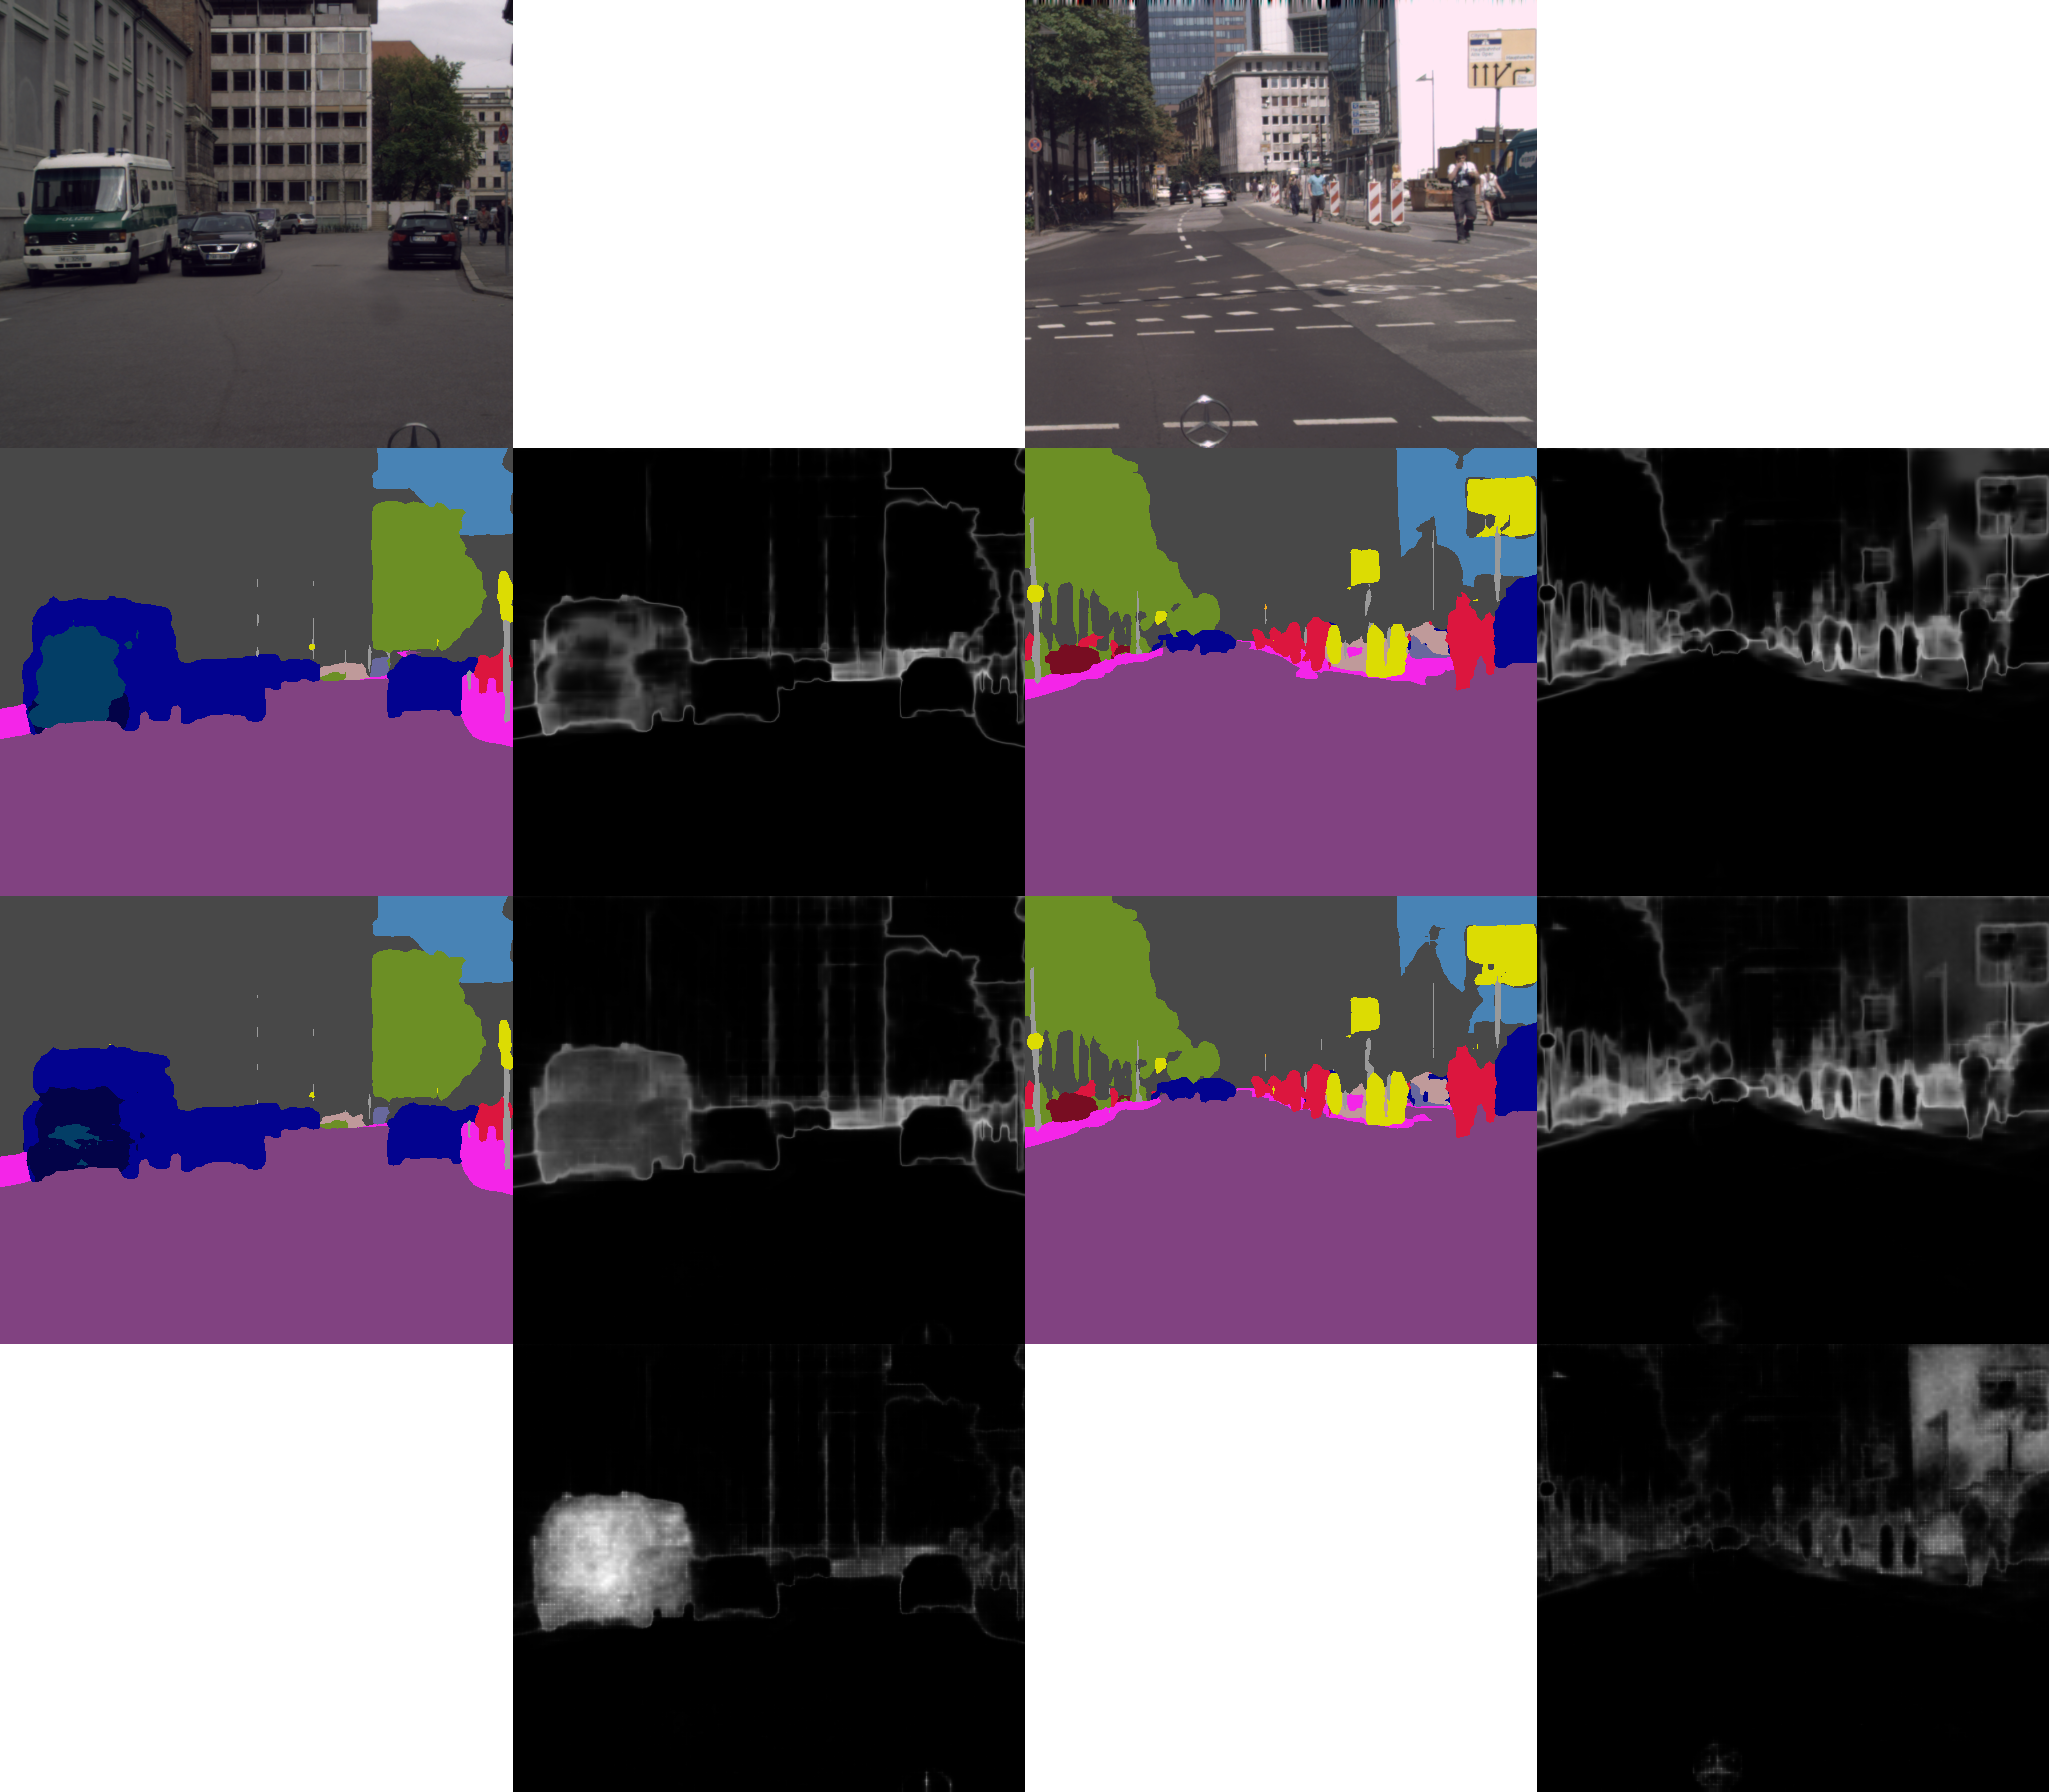
\includegraphics[height=6.4cm,keepaspectratio]{experiments/uncertainty-predictions-cityscapes-mini.png}}
		\raisebox{0\height+0cm}{
		\hspace*{-0.2cm}\begin{minipage}[b][6.4cm]{1cm}\offinterlineskip
			\tiny
			\begin{tabu} {@{}X[1,c,m]@{}@{}X[-1,c,m]@{}}
				\makecell[l]{} & \vspace{1.6cm} \\
				\makecell[l]{entropija --\\ \textit{dropout}} &\vspace{1.6cm} \\
				\makecell[l]{$U_\text{A}$} &\vspace{1.6cm} \\
				\makecell[l]{$U_\text{E} \cdot 4$ } &\vspace{1.6cm}
			\end{tabu}
		\end{minipage}
		}
		\hspace*{-0.4cm}\raisebox{0\height-0cm}{%
		\begin{minipage}[b][6.3579cm]{2.0cm}\offinterlineskip
			\resizebox{0.67\textwidth}{!}{%
			\scriptsize
			\begin{minipage}[b]{1.5cm}\offinterlineskip
				\begin{tabu} {@{}X[1,r,m]@{} @{}X[-1,c,m]@{}}
					neoznačeno &\vspace{0.5cm} \\
					cesta &\vspace{0.5cm} \\
					nogostup &\vspace{0.5cm} \\
					građevina &\vspace{0.5cm} \\
					zid &\vspace{0.5cm} \\
					ograda &\vspace{0.5cm} \\
					stup &\vspace{0.5cm} \\
					semafor &\vspace{0.5cm} \\
					prom.~znak &\vspace{0.5cm} \\
					vegetacija &\vspace{0.5cm} \\			
					teren &\vspace{0.5cm} \\			
					nebo &\vspace{0.5cm} \\			
					čovjek &\vspace{0.5cm} \\			
					biciklist &\vspace{0.5cm} \\
					automobil &\vspace{0.5cm} \\
					kamion &\vspace{0.5cm} \\			
					autobus &\vspace{0.5cm} \\			
					vlak &\vspace{0.5cm} \\	
					motocikl &\vspace{0.5cm} \\	
					bicikl &\vspace{0.5cm} \\
				\end{tabu}
			\end{minipage}
			\raisebox{-.5\height+0.85mm}{
\includegraphics[height=10cm,keepaspectratio]{experiments/cityscapes-colors.png}}
			}
		\end{minipage}
		}
		}}
\end{frame}
\note[itemize]{
	\item\item 0.40 / 13:00
}

\begin{frame}{}
\vspace*{-3cm}\raisebox{0cm}{
	\centering
	\resizebox{1.1\textwidth}{!}{%
		\hspace*{-0.8cm}\begin{minipage}[b]{1.2cm}\offinterlineskip
			\tiny
			\begin{tabu} {@{}X[1,c,m]@{}@{}X[-1,c,m]@{}}
				\makecell[r]{ulaz} & \vspace{1.6cm} \\
				\makecell[r]{predikcija --\\ \textit{dropout}} & \vspace{1.6cm} \\
				\makecell[r]{predikcija --\\ \textit{MC-dropout}} &\vspace{1.6cm} \\	
				\makecell[r]{} &\vspace{1.6cm} \\
			\end{tabu}
		\end{minipage}
		\raisebox{-.5\height+0.85mm}{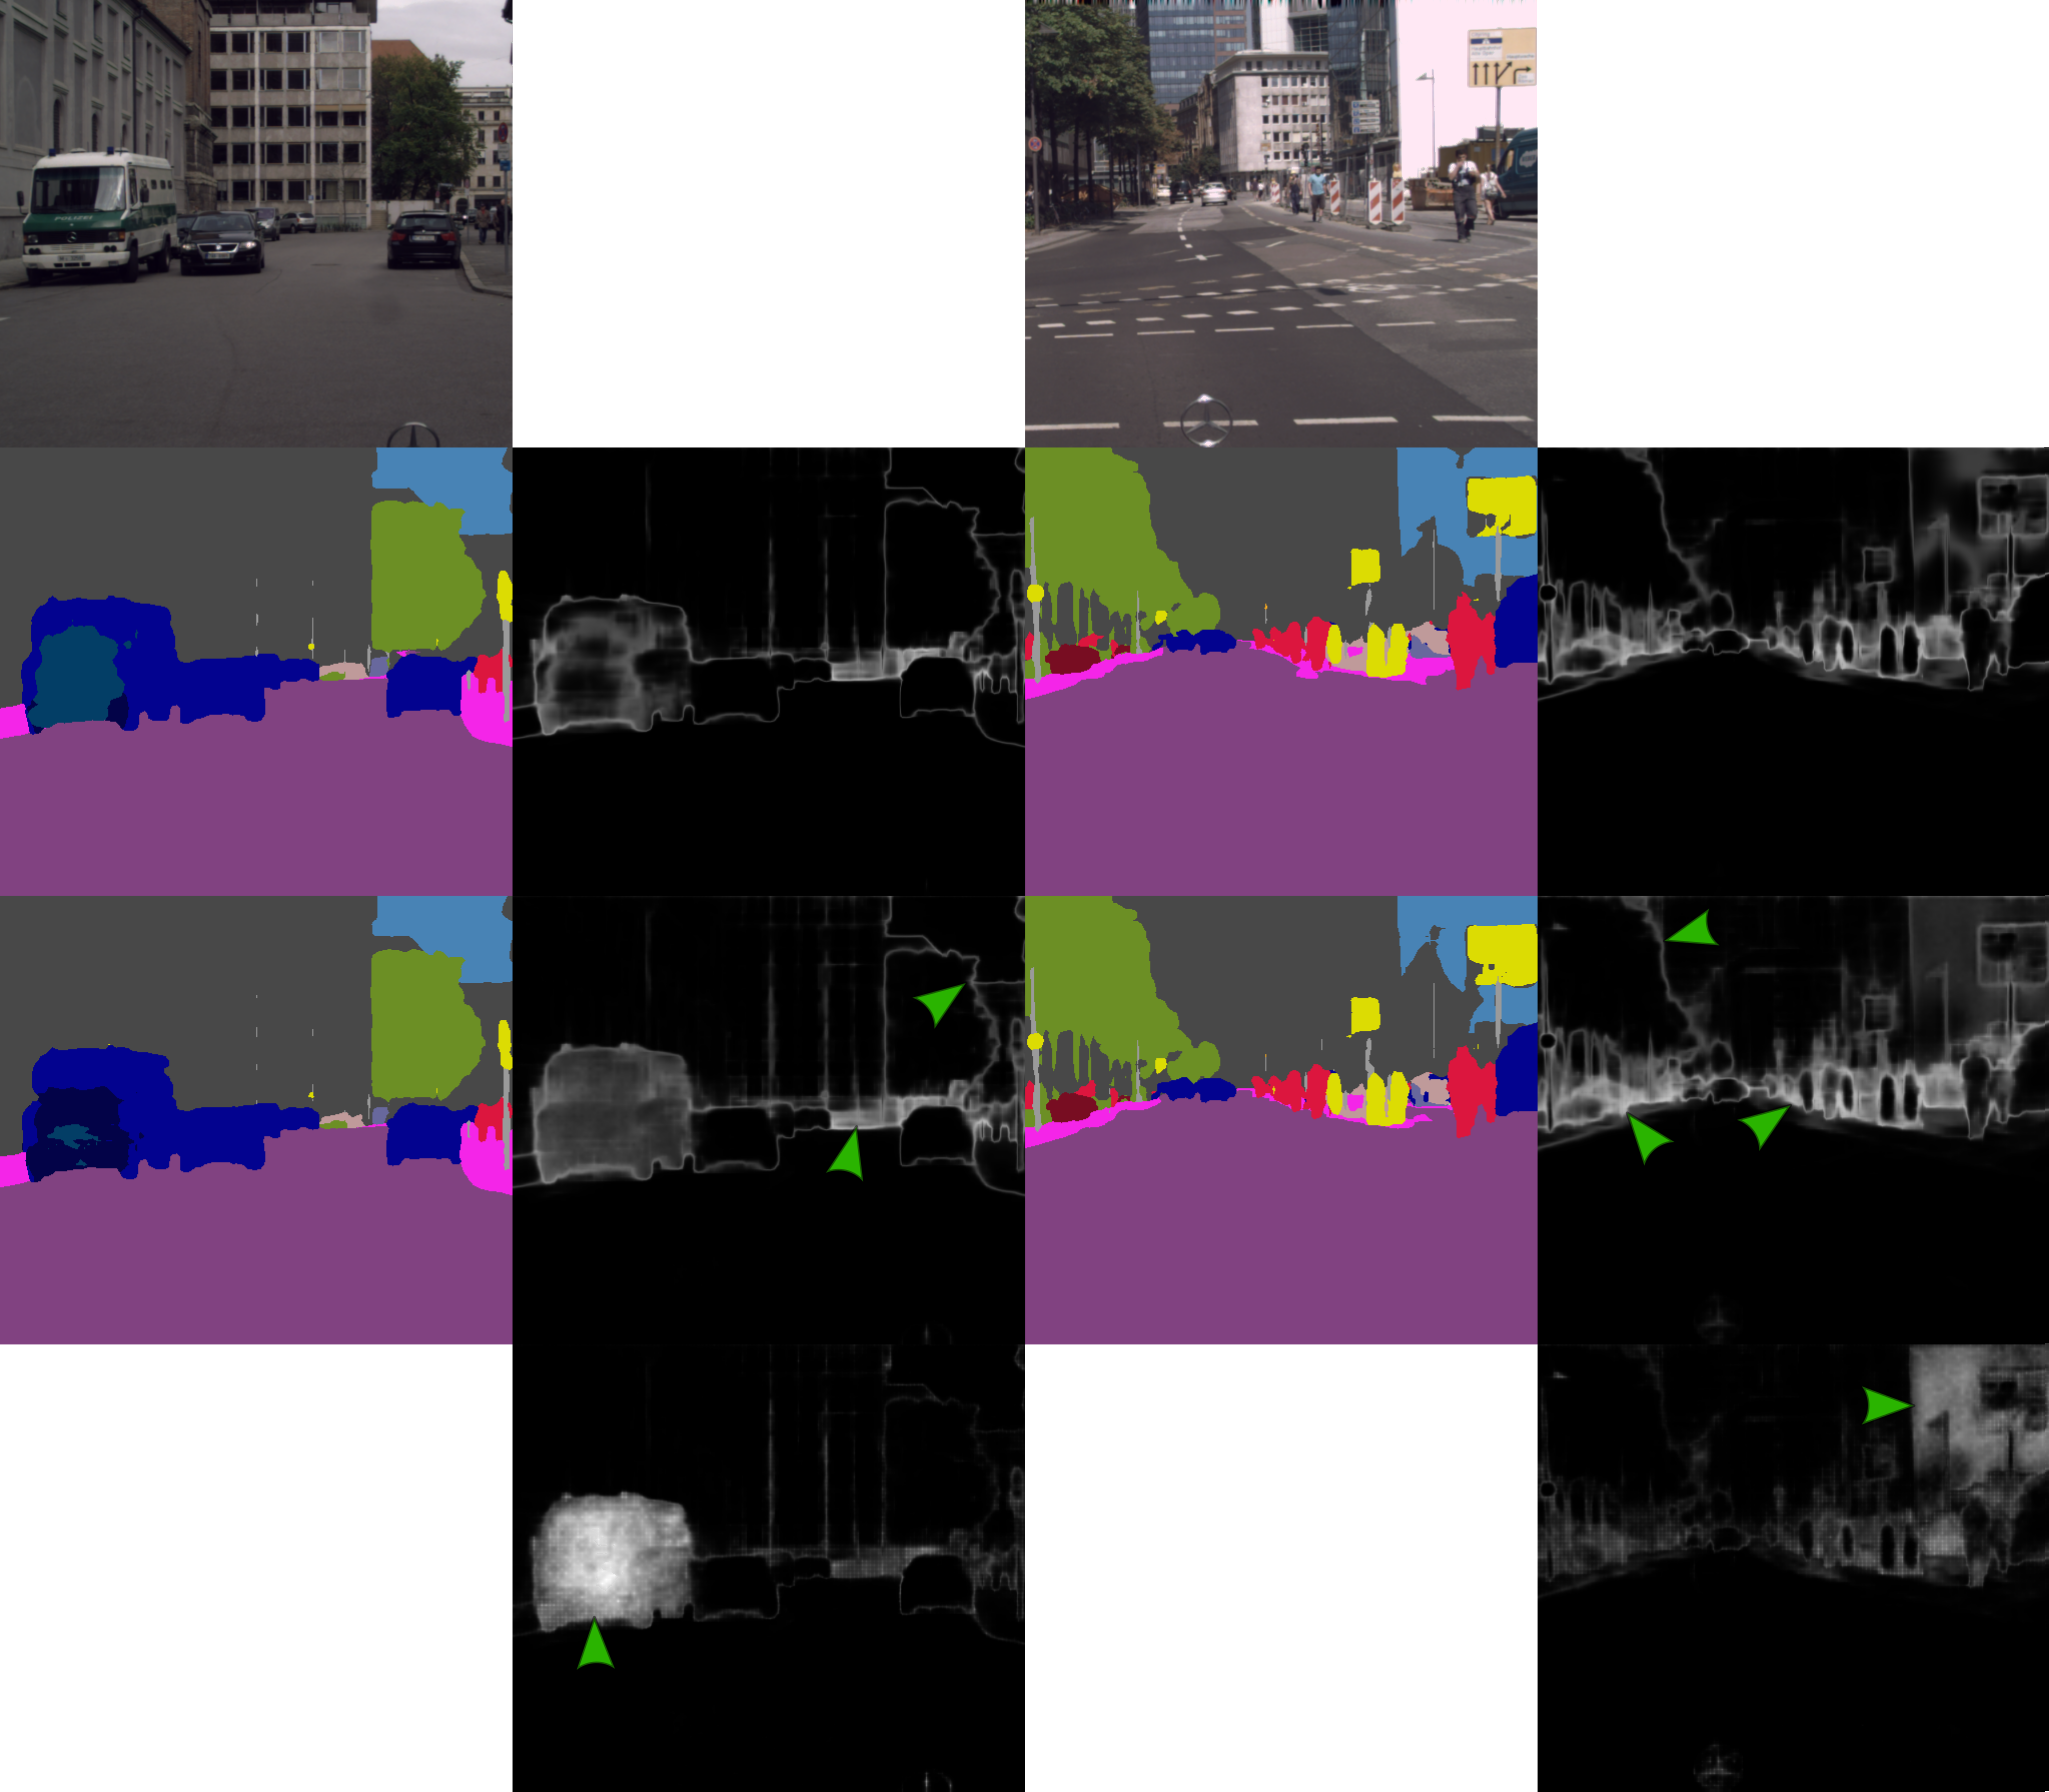
\includegraphics[height=6.4cm,keepaspectratio]{experiments/uncertainty-predictions-cityscapes-mini-annot.png}}
		\raisebox{0\height+0cm}{
			\hspace*{-0.2cm}\begin{minipage}[b][6.4cm]{1cm}\offinterlineskip
				\tiny
				\begin{tabu} {@{}X[1,c,m]@{}@{}X[-1,c,m]@{}}
					\makecell[l]{} & \vspace{1.6cm} \\
					\makecell[l]{entropija --\\ \textit{dropout}} &\vspace{1.6cm} \\
					\makecell[l]{$U_\text{A}$} &\vspace{1.6cm} \\
					\makecell[l]{$U_\text{E} \cdot 4$ } &\vspace{1.6cm}
				\end{tabu}
			\end{minipage}
		}
		\hspace*{-0.4cm}\raisebox{0\height-0cm}{%
			\begin{minipage}[b][6.3579cm]{2.0cm}\offinterlineskip
				\resizebox{0.67\textwidth}{!}{%
					\scriptsize
					\begin{minipage}[b]{1.5cm}\offinterlineskip
						\begin{tabu} {@{}X[1,r,m]@{} @{}X[-1,c,m]@{}}
							neoznačeno &\vspace{0.5cm} \\
							cesta &\vspace{0.5cm} \\
							nogostup &\vspace{0.5cm} \\
							građevina &\vspace{0.5cm} \\
							zid &\vspace{0.5cm} \\
							ograda &\vspace{0.5cm} \\
							stup &\vspace{0.5cm} \\
							semafor &\vspace{0.5cm} \\
							prom.~znak &\vspace{0.5cm} \\
							vegetacija &\vspace{0.5cm} \\			
							teren &\vspace{0.5cm} \\			
							nebo &\vspace{0.5cm} \\			
							čovjek &\vspace{0.5cm} \\			
							biciklist &\vspace{0.5cm} \\
							automobil &\vspace{0.5cm} \\
							kamion &\vspace{0.5cm} \\			
							autobus &\vspace{0.5cm} \\			
							vlak &\vspace{0.5cm} \\	
							motocikl &\vspace{0.5cm} \\	
							bicikl &\vspace{0.5cm} \\
						\end{tabu}
					\end{minipage}
					\raisebox{-.5\height+0.85mm}{
\includegraphics[height=10cm,keepaspectratio]{experiments/cityscapes-colors.png}}
				}
			\end{minipage}
		}
}}
\end{frame}
\note[itemize]{
	\item\item 1.00 / 14:00
}

\section{Eksperimenti: prepoznavanje izvanrazdiobnih primjera}

\begin{frame}{Eksperimenti: prepoznavanje izvanrazdiobnih primjera}
\begin{itemize}
\item \citet{Liang:2017:PDOODENN} pokazuju da su veće temperature bolje, pa se u eksperimentima s temperaturnim skaliranjem koristi $T=1000$.
\item Kao pozitivna klasa se uzimaju unutarrazdiobni primjeri.
\item Za svaki izvanrazdiobni skup se izdvaja $10\%$ slika za odabir parametra pomaka $\epsilon$ minimizacijom $\FPR$-a (učestalosti klasifikacije negativnih primjera kao pozitivnih) kad je odziv $R=0.95$. 
\item  Ispitani su postupci klasifikacije:
\begin{enumerate}
	\item po najvećoj vrijednosti softmaksa uz $T=1$ \citep{Hendrycks:2016:BDMOODE}
	\item po najvećoj vrijednosti softmaksa uz $T=1000$ \citep{Liang:2017:PDOODENN}
	\item po najvećem logitu
	\item po najvećem normaliziranom logitu
	\item logističkom regresijom po zbroju i maksimalnoj vrijednosti logita
	\item logističkom regresijom po zbroju i maksimalnoj vrijednosti normaliziranih logita
\end{enumerate}
uz i bez FGSM-a.
\end{itemize}
\end{frame}
\note[itemize]{
	\item Kao pozitivna klasa se uzimaju unutarrazdiobni primjeri.
	\item Za svaki izvanrazdiobni skup se izdvaja $10\%$ slika za odabir parametra pomaka $\epsilon$ minimizacijom $\FPR$-a kad je odziv $R=0.95$. 
	\item  Ispitani su postupci klasifikacije (uz i bez FGSM-a):
	\begin{enumerate}
		\item po najvećoj vrijednosti softmaksa uz $T=1$ \citep{Hendrycks:2016:BDMOODE}
		\item .. uz $T=1000$ \citep{Liang:2017:PDOODENN}
		\item po najvećem logitu
		\item po najvećem normaliziranom logitu
		\item logističkom regresijom po zbroju i maksimalnoj vrijednosti logita
		\item logističkom regresijom po zbroju i maksimalnoj vrijednosti normaliziranih logita
	\end{enumerate}
	uz i bez FGSM-a.
	\item\item 0.50 / 14:50
}

\begin{frame}{}	
\begin{table}
	\centering\footnotesize
	\begin{tabular}{l|rr}
		\toprule
		$\AUROC/\%$ & \makecell[l]{DN-100-12\\ ($A=0.948$)} & \makecell[l]{WRN-28-10\\ ($A=0.957$)} \\
		\midrule
		najveća vjerojatnost & $92.4$ & $90.5$ \\
		najveća vjerojatnost, $T=1000$ & $95.7$ & $93.1$ \\
		najveća vjerojatnost, $T=1000$, FGSM & $96.5$ & $95.3$ \\
		najveći logit & $96.3$ & $93.3$ \\
		najveći logit, FGSM & $96.5$ & $95.3$ \\
		\midrule
		najveći logit, FGSM & $96.2$ & $95.1$ \\
		logistička regresija & $96.4$ & $95.5$ \\
		logistička regresija, FGSM & $97.0$ & $95.5$ \\
		najveći normalizirani logit & $97.5$ & $96.8$ \\
		najveći normalizirani logit, FGSM & $97.7$ & $96.6$ \\
		logistička regresija i normalizirani logiti & $97.7$ & $96.9$ \\
		logistička regresija i normalizirani logiti, FGSM & $97.8$ & $96.9$ \\
		\bottomrule
	\end{tabular}
	\caption{Prosječni $\AUROC$ na skupovima TinyImagenet-C, TinyImagenet-R, LSUN-C, LSUN-R, iSUN, \textit{uniformni šum}, \textit{gaussov šum}. Sufiks \textit{C} znači da su nasumično izrezani dijelovi slika, a \textit{R} da su slike smanjene na dimenzije $32\times32$.}
\end{table}
\end{frame}
\note[itemize]{
	\item\item 2.20 / 16:10
}

\begin{frame}{}
\begin{figure}
	\centering
	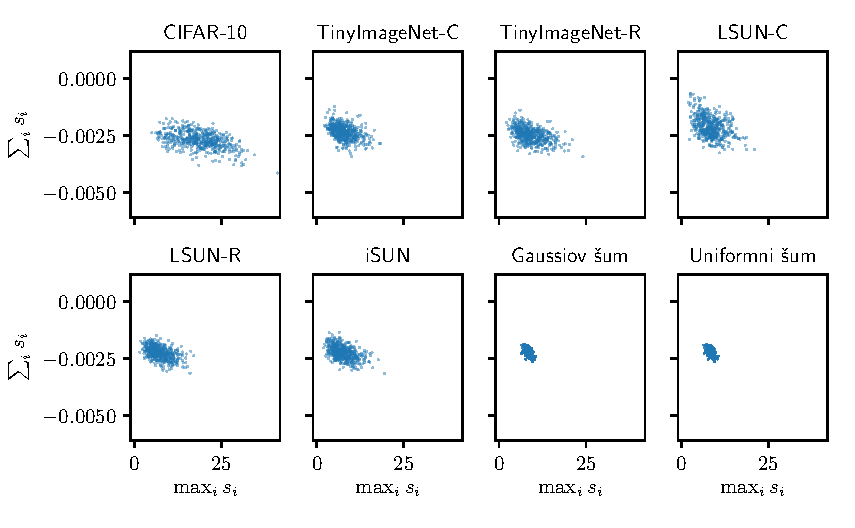
\includegraphics[width=1\textwidth]{dn-100-12-maxlogits-sumlogits}
	\caption{Odnos maksimalnog logita i zbroja logita za različite skupove kod mreže DenseNet-100-12.}
	\label{fig:dn-100-12-maxlogits-sumlogits}
\end{figure}
\end{frame}
\note[itemize]{
	\item\item 0.40 / 17:50
}


\section{Zaključak}

\begin{frame}{Zaključak}
\begin{itemize}
	\item Rezultati procjenjivanja epistemičke i  aleatorne nesigurnosti uglavnom nisu u skladu s očekivanjem. Bilo bi dobro pokušati ih bolje razumjeti.
	\item Rezultati prepoznavanja izvanrazdiobnih primjera pokazuju da se performansa može poboljšati klasifikacijom na temelju većeg broja značajki izvedenih iz vektora logita.
\end{itemize}
\end{frame}
\note[itemize]{
	\item Rezultati procjenjivanja epistemičke i  aleatorne nesigurnosti uglavnom nisu u skladu s očekivanjem. Bilo bi dobro pokušati ih bolje razumjeti.
	\item Rezultati prepoznavanja izvanrazdiobnih primjera pokazuju da se performansa može poboljšati klasifikacijom na temelju većeg broja značajki izvedenih iz vektora logita.
	\item\item 0.20 / 18:10
}

\begin{frame}[allowframebreaks=0.95]
\frametitle{Literatura}
	\bibliography{literatura}
	\bibliographystyle{fer} 
\end{frame}


\begin{frame}{Međusobna informacija kao mjera epistemičke nesigurnosti}
\begin{itemize}
\item Tu međusobnu informaciju možemo i ovako izraziti:
\begin{align}
\I\del{\del{\rvar y\mid\vec x,\set D};\del{\rvec\theta\mid\set D}}
&= \H(\rvec\theta\mid\set D) - \H\del{\del{\rvec\theta\mid\set D}\mid\del{\rvar y\mid\vec x,\set D}} \\
&= \H(\rvec\theta\mid\set D) - \H\del{\del{\rvec\theta\mid\vec x,\set D}\mid\del{\rvar y\mid\vec x,\set D}} \\
&= \H(\rvec\theta\mid\set D) - \E_{\rvar y\mid\vec x,\set D} \H(\rvec\theta\mid\vec x,y,\set D) \text{.} \label{eq:mi-epistemicka-nesigurnost-2}
\end{align}
\item Zadnji izraz je razlika entropije aposteriorne razdiobe parametara i očekivanja entropije aposteriorne razdiobe parametara ako se u podatke uključi označeni primjer $\vec x$.
\item To možemo interpretirati kao očekivano znanje o parametrima koje dobijemo ako dobijemo oznaku za primjer $\vec x$.
\end{itemize}
\end{frame}

\begin{frame}{Aproksimacija bayesovske neuronske mreže pomoću dropouta}
\begin{figure}
	\centering
	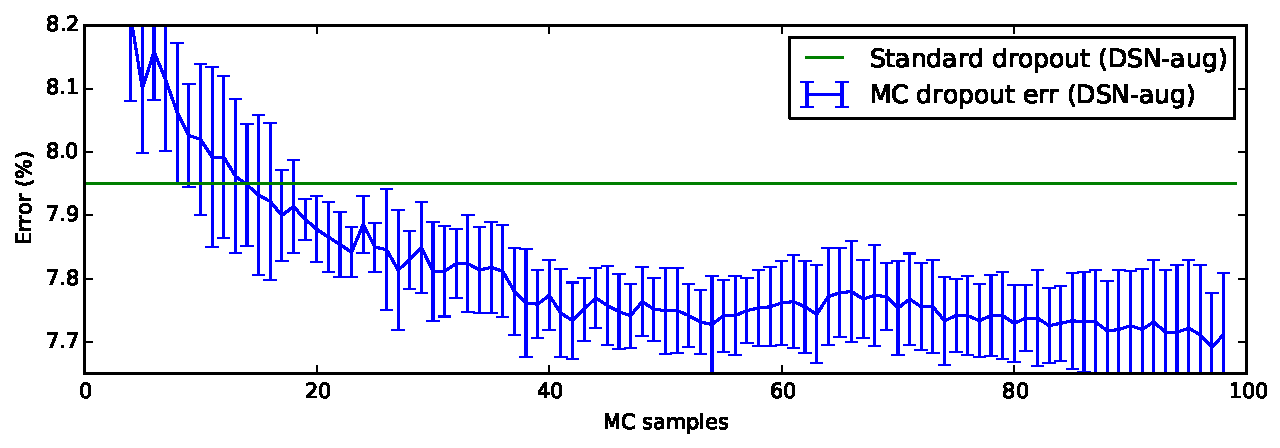
\includegraphics[width=1.0\textwidth]{uncertainty/DSN_samples}
	\caption{Ovisnost klasifikacijske pogreške (plavo) o broju uzoraka u \textit{Monte Carlo} aproksimaciji izlaza na konvolucijskoj mreži koju su ispitivali autori \citep{Gal:2016:BCNNBAVI} na skupu CIFAR-10. Svaka točka je prosjek $5$ mjerenja i prikazane su standardne devijacije. Zeleni pravac označava klasifikacijsku pogrešku kod uobičajenog usrednjavanja skaliranjem težina. Slika je preuzeta iz \citet{Gal:2016:BCNNBAVI}.}
	\label{fig:mc-drouput-samples-DSN}
\end{figure}
\end{frame}

\begin{frame}[shrink]{}
\begin{minipage}[b]{1.4\textwidth}
\begin{figure}
	\centering
	\begin{subfigure}[t]{1\textwidth}
		\centering
		\begin{tikzpicture}
		\node[nrect] (x) [] {$\vec x$};
		\node[nrect] (g) [right=of x] {$g$};
		\node[above=0mm of g] {$\vec s$};
		\node[nrect] (t) [right=of g] {$\frac{1}{T}\phbox$};
		\node[nrect] (y) [right=of t] {$\softmax$};
		\node[above=0mm of y] {$\hat{\vec y}$};
		\node[nrect] (max) [right=of y] {$\max_k \phbox_\ind{k}$};
		\node[nrect] (clf) [right=of max] {$D$};
		\path (x) edge [dedge] (g);
		\path (g) edge [dedge] (t);
		\path (t) edge [dedge] (y);
		\path (y) edge [dedge] (max);
		\path (max) edge [dedge] (clf);
		\end{tikzpicture}
		\caption{Klasifikacija po maksimalnoj vrijednosti softmaksa.}
		\label{subfig:graf-ood-softmax-temp}
	\end{subfigure}

	\begin{subfigure}[t]{1\textwidth}
		\centering
		\begin{tikzpicture}
		\node[nrect] (x) [] {$\vec x$};
		\node[nrect] (g) [right=of x] {$g$};
		\node[above=0mm of g] {$\vec s$};
		\node[nrect] (max) [right=of g] {$\max_k \phbox_\ind{k}$};
		\node[nrect] (clf) [right=of max] {$D$};
		\path (x) edge [dedge] (g);
		\path (g) edge [dedge] (max);
		\path (max) edge [dedge] (clf);
		\end{tikzpicture}
		\caption{Klasifikacija po maksimalnom logitu.}
		\label{subfig:graf-ood-logiti}
	\end{subfigure}

	\begin{subfigure}[t]{1\textwidth}
		\centering
		\begin{tikzpicture}
		\node[nrect] (x) [] {$\vec x$};
		\node[nrect] (g) [right=of x] {$g$};
		\node[above=0mm of g] {$\vec s$};
		\node[nrect] (n) [right=of g] {$N$};
		\node[nrect] (max) [right=of n] {$\max_k \phbox_\ind{k}$};
		\node[nrect] (clf) [right=of max] {$D$};
		\path (x) edge [dedge] (g);
		\path (g) edge [dedge] (n);
		\path (n) edge [dedge] (max);
		\path (max) edge [dedge] (clf);
		\end{tikzpicture}
		\caption{Klasifikacija po maksimalnom normaliziranom logitu.}
		\label{subfig:graf-ood-normalizacija}
	\end{subfigure}

	\begin{subfigure}[t]{1\textwidth}
		\centering
		\begin{tikzpicture}
		\node[nrect] (x) [] {$\vec x$};
		\node[nrect] (g) [right=of x] {$g$};
		\node[above=0mm of g] {$\vec s$};
		\node[nrect] (ms) [right=of g] {$\sbr{\max_k \phbox_\ind{k}, \sum_k \phbox_\ind{k}}$};
		\node[above=0mm of ms] {$\vec z$};
		\node[nrect] (msn) [right=of ms] {$N$};
		\node[nrect] (pf) [right=of msn] {$\phi$};
		\node[nrect] (lr) [right=of pf] {$\sigma(\vec w^\tp\phbox)$};
		\node[nrect] (clf) [right=of lr] {$D$};
		\path (x) edge [dedge] (g);
		\path (g) edge [dedge] (ms);
		\path (ms) edge [dedge] (msn);
		\path (msn) edge [dedge] (pf);
		\path (pf) edge [dedge] (lr);
		\path (lr) edge [dedge] (clf);
		\end{tikzpicture}
		\caption{Klasifikacija para koji čine maksimalni logit i zbroj logita logističkom regresijom s normalizacijom i polinomijalnim baznim funkcijama stupnjeva od $0$ do $2$.}
		\label{subfig:graf-ood-logreg}
	\end{subfigure}

	\begin{subfigure}[t]{1\textwidth}
		\centering
		\begin{tikzpicture}
		\node[nrect] (x) [] {$\vec x$};
		\node[nrect] (g) [right=of x] {$g$};
		\node[above=0mm of g] {$\vec s$};
		\node[nrect] (n) [right=of g] {$N$};
		\node[nrect] (ms) [right=of n] {$\sbr{\max_k \phbox_\ind{k}, \sum_k \phbox_\ind{k}}$};
		\node[above=0mm of ms] {$\vec z$};
		\node[nrect] (msn) [right=of ms] {$N$};
		\node[nrect] (pf) [right=of msn] {$\phi$};
		\node[nrect] (lr) [right=of pf] {$\sigma(\vec w^\tp\phbox)$};
		\node[nrect] (clf) [right=of lr] {$D$};
		\path (x) edge [dedge] (g);
		\path (g) edge [dedge] (n);
		\path (n) edge [dedge] (ms);
		\path (ms) edge [dedge] (msn);
		\path (msn) edge [dedge] (pf);
		\path (pf) edge [dedge] (lr);
		\path (lr) edge [dedge] (clf);
		\end{tikzpicture}
		\caption{Klasifikacija para koji čine maksimalni normalizirani logit i zbroj normaliziranih logita logističkom regresijom s normalizacijom i polinomijalnim baznim funkcijama sa stupnjevima od $0$ do $2$.}
		\label{subfig:graf-ood-normalizacija-logreg}
	\end{subfigure}
	\caption{Grafički prikaz postupaka za klasifikaciju na temelju logita ili softmaksa. $g\colon\vec x\mapsto\vec s$ je funkcija koja ulaz preslikava u vektor logita. $N$ je funkcija koja normalizira vektor po svakoj komponenti posebno oduzimanjem sredine i dijeljenjem sa standardnom devijacijom prema izdvojenim skupovima. $\phi\colon\sbr{a,b}\mapsto\sbr{1,a,b,a^2,b^2,ab}$ je funkcija polinomijalnih značajki sa stupnjevima od $0$ do $2$. $D$ je funkcija koja određuje pripada li primjer razdiobi skupa za učenje usporedbom ulaza s pragom.}
	\label{fig:ood-racunski-grafovi}
\end{figure}
\end{minipage}
\end{frame}
\end{document}
